\documentclass[11pt]{article}
\usepackage[a4paper,margin=24mm]{geometry}
\usepackage{amsmath,amssymb,graphicx,booktabs,longtable,hyperref,iftex,cite}
\ifXeTeX
\usepackage{fontspec}
\setmainfont{texgyretermes-regular.otf}[BoldFont=texgyretermes-bold.otf,ItalicFont=texgyretermes-italic.otf,BoldItalicFont=texgyretermes-bolditalic.otf]
\fi
\title{LEG-SEIR: Implementation, Evidence and Reproduction Supplement}
\author{Anonymous Authors}
\date{}
\makeatletter
\newcommand{\bstctlcite}[1]{\immediate\write\@auxout{\string\citation{#1}}}
\makeatother
\begin{document}\bstctlcite{BSTcontrol}\emergencystretch=2em\setlength{\tabcolsep}{4pt}\maketitle
\section{Scope and evidence boundaries}
This supplement accompanies the six-page LEG-SEIR manuscript. It documents the evaluated computation, full comparison, source provenance and remaining tests. It does not turn a retrospective case study into prospective confirmation. The proposed name is provisional; scientific priority for the complete combination is not established. The public code repository and Hugging Face release provide audited tables and recorded experiment evidence. Original third-party source PDFs are retained separately; source URLs and retrieval hashes are public.

The frozen scientific notebook has code SHA256
\begin{center}\small\texttt{3ea0794104f30993d7b0994c17e76e95435def0ad11305cfa535c91828009ed1}\end{center}
and the source manifest identity is
\begin{center}\small\texttt{69332f61488130cdf730e08a06f4ab417742c6b57834815d812ca7903662f239}.\end{center}
Hash identity is distinct from clinical accuracy, experimental independence or deterministic bitwise reruns. The package includes its own manifest and copy origins.

\section{Data reconstruction and chronology}
The original case publisher is the Epidemiology Unit, Ministry of Health, Sri Lanka. Population tables are from the Department of Census and Statistics. The version-one curated source snapshot used for the Kaggle execution, provides an execution/distribution snapshot; it is not the original publisher. Its 714-entry source manifest covers report PDFs, population files and pinned ancillary files. Exact source URLs, byte hashes and retrieval status are included in the archive. The main model uses case histories and constant Census 2012 scaling only. GADM and ERA5 materials are preserved for provenance but are not additional forecast inputs in this experiment.

There are 686 report slots, 663 finite 25-district rows and 23 missing rows under the frozen primary policy. Weekly row A and cumulative row B are parsed from original PDFs with layout-specific handling. Arithmetic checks and reconstruction decisions are recorded rather than silently replacing source values. Ampara and Kalmunai reporting divisions are aggregated into one district. Generic unresolved-repeat handling applies to historical reports; no extreme count is removed on the basis of model error. Missing windows are excluded, not interpolated or zero-filled.

\begin{center}
\begin{tabular}{lrrr}\toprule Stage & Training origins & Validation origins & Test origins\\\midrule
Development 2023 &447&30&--\\
Development 2025 &525&40&--\\
Final retrospective 2026 &525&40&18\\\bottomrule\end{tabular}
\end{center}
Training targets precede the validation year; all horizon targets for a validation/test origin belong to its declared year. Input histories may include earlier years or earlier observed test reports. Train/validation/test target observations are disjoint. Rounded final scaler mean/std are 2.663785 and 1.515723; the 2023 fold values are 2.575081 and 1.529113. Full precision is preserved in checkpoints. Statistics use unique observations touched by training inputs and targets. A new run must compute them from the data rather than impose them as fitting inputs.

The archive ends at Vol. 53 No. 33 and is not a complete 2026 calendar year. Report-period years do not supply historical immutable release vintages. Complete-window exclusion changes coverage; this study does not quantify how performance would change if every unresolved report were accepted. The alternative printed-repeat series is archived, but the LEG-SEIR experiment did not train or score that alternative policy.

\section{Function-level implementation map}
\begin{longtable}{p{.27\textwidth}p{.65\textwidth}}\toprule Function & Role and important details\\\midrule
\texttt{read\_table1} and parser helpers & Find the district dengue A/B rows in normal and rotated layouts. District header aliases are normalized; parsing failure is recorded.\\
\texttt{adjacency} & Receiver/sender factor products, self-edge masking, top-five selection and row-softmax. No geography or measured mobility is consumed.\\
\texttt{base\_hidden} & Concatenate three standardized levels and two consecutive differences; apply Linear(5,64), ReLU, Linear(64,64), ReLU. The proposed configuration has no district-ID input.\\
\texttt{lag\_weights} & Softmax of a learned 25-by-3 logit matrix; each receiver has one lag distribution shared across all senders and origins.\\
\texttt{imported} & Divide raw history by population/11, clip, apply graph aggregation, then lag weighting and summation. Returns one historical pressure anchor per district.\\
\texttt{exposure\_forecast} & Initialize normalized proxy states; compute positive horizon rates; blend decaying historical and simulated neighbour pressure; blend imported/local pressure; execute 21 conservative daily steps; sum onset flows in groups of seven.\\
\texttt{conservative\_step} & Compute bounded S-to-E, E-to-I and I-to-R outflows from the pre-update state. Return the next state and E-to-I flow.\\
\texttt{forward} & Encode local and lag-weighted neighbour histories; form gated residual graph message; compute shared local/graph readouts and a separate rate head; transform SEIR counts to standardized logs; mix four experts.\\
\texttt{routing\_weights} & Horizon softmax logits of shape 3-by-4, broadcast over districts and batches. No input-conditioned routing is used.\\
\texttt{fit} & Seed, shuffle, minimize log MSE with Adam, clip gradients, choose the lowest validation count RMSE checkpoint, export curves/checkpoint, and check CPU reload parity before accepting selection evidence.\\
\texttt{baseline} & Repeat the latest observed district count on the same eligible forecast origins; export targets and predictions.\\
\texttt{ridge\_baseline} & Fit pooled multi-output ridge at fixed alpha=1 to three standardized levels and two differences. No alpha search is performed.\\
\texttt{verify} & ZIP/hash and code identities; raw target/scaler reconstruction; split chronology; count/horizon metrics; checkpoint minima; CPU neural output parity; development-based LR selection and final control settings. Does not refit ridge or validate epidemiological mechanisms.\\\bottomrule
\end{longtable}

The modular source snapshot is included for reading. The exact submitted notebook embeds all scientific runtime code; it is the authoritative executable artifact. A results-gallery notebook is separately labelled because reading saved outputs is not training from scratch.

\section{Hyperparameters and non-learned assumptions}
\begin{center}\begin{tabular}{ll}\toprule Quantity & Evaluated value\\\midrule
Input/output history &3 reports / 3 horizons\\
Shared MLP &5 inputs, width 64, two ReLU layers\\
Adjacency factors &25-by-8 each; 5 non-self senders per receiver\\
Lag logits &25-by-3; zero initialized\\
Graph/import gates &Scalar sigmoid, logit initialized at -2\\
Mixture logits &3-by-4; zero initialized\\
SEIR population scale &Census 2012 / 11\\
Initial susceptible proxy &0.318, followed by mass normalization\\
Initial E/I &Previous/latest count divided by scale; clipped to $[10^{-6},0.5]$\\
Exposed/recovery rate &$\omega=.1$, $\gamma=1/7$\\
Pressure decay &Fixed $\tau=7$ solver days\\
Daily rollout &7 steps per horizon, 21 steps in total\\
Transmission transform &$\exp(\operatorname{clip}(r-1.1,-9,1.1))$\\
Training &Adam; batch 128; clip gradient norm 5\\
Weight decay &$10^{-4}$, except adapter-specific exemption in that baseline\\
Budget &300 epochs maximum, early stopping patience 40\\
Development LR grid &0.001, 0.003; seeds 0,1,2\\
Final seeds &0,1,2,3,4\\\bottomrule\end{tabular}\end{center}
Rates and states are unvalidated proxies. The fixed scale, initialization and daily-to-report mapping were inherited rather than identified from clinical measurements. Human-only SEIR is not a complete dengue vector-host model. Fixed-constant sensitivity is a remaining experiment, not a completed robustness finding.

\section{Full final comparisons}
All primary final neural configurations use five seeds and the same 18 origins. Parent-selected LR is used for removals. Configuration names below preserve the exact experiment registry; \texttt{lagged\_full} is LEG-SEIR. \texttt{observer\_full} is the compartment-only variant without state features. \texttt{observer\_seir\_off} is an ordinary neural horizon mixture because removing its compartment mechanism leaves no observer operation.
\footnotesize\begin{longtable}{lrrrrr}\toprule Configuration & LR & Parameters & Mean RMSE & SD & MAE\\\midrule
horizon\_full & 0.001 & 9443 & 81.748689 & 1.282886 & 32.681789\\
horizon\_graph\_off & 0.001 & 4946 & 83.977142 & 2.204693 & 33.633430\\
horizon\_seir\_off & 0.001 & 9443 & 81.362749 & 0.607761 & 32.477848\\
identity\_mlp & 0.001 & 5095 & 81.392283 & 0.717613 & 32.504498\\
lagged\_full & 0.003 & 9519 & 79.634330 & 0.636198 & 32.141853\\
lagged\_graph\_off & 0.003 & 4946 & 84.157640 & 2.861065 & 33.518708\\
lagged\_seir\_off & 0.003 & 9518 & 81.263732 & 0.569785 & 32.868093\\
local\_mlp & 0.003 & 4739 & 84.859119 & 1.393745 & 33.802822\\
local\_seir & 0.003 & 4940 & 84.891959 & 3.174829 & 33.719131\\
observer\_full & 0.003 & 9703 & 81.760844 & 1.588469 & 32.881089\\
observer\_graph\_off & 0.003 & 5206 & 83.768908 & 1.968693 & 33.327539\\
observer\_seir\_off & 0.003 & 9443 & 82.116504 & 1.316723 & 33.103233\\
plain\_graph & 0.003 & 9236 & 82.633195 & 1.019258 & 33.229765\\
shared\_adapter & 0.001 & 10476 & 80.756884 & 0.383053 & 32.454080\\
uniform\_mixture & 0.003 & 9431 & 83.145236 & 4.171663 & 33.194150\\
\bottomrule\end{longtable}\normalsize
Persistence RMSE is 87.382382; shared ridge is 85.543142. Secondary metrics and individual seed/horizon scores are available in the complete CSV. The final study contains 350 scored neural rows (development validation and final validation/test records), not 350 independent fits.

Horizon graph-off and SEIR-off have own development-selected LR 0.003 instead of their parent's 0.001. Their additional five-seed sensitivities give mean test RMSE 84.157640 and 82.116504. They are not substituted for the primary parent-LR controls. All other matched removals retain 0.003 under both conventions.

\section{Forecast visualization and learned diagnostics}
\begin{figure}[ht]\centering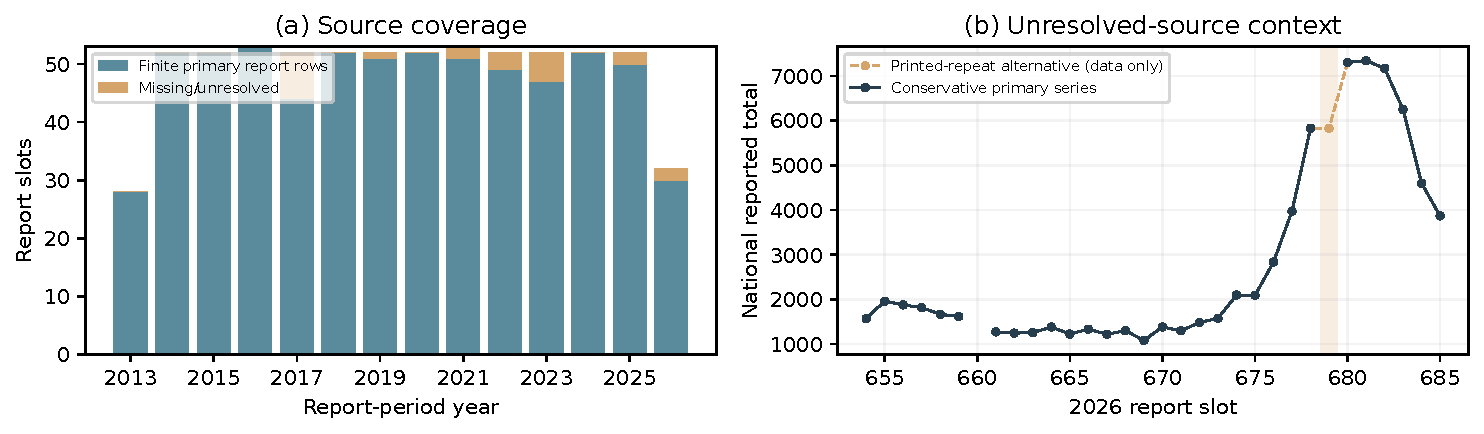
\includegraphics[width=\textwidth]{figures/source_coverage.pdf}
\caption{Source coverage and reporting uncertainty. The alternative printed-repeat series is shown as source context only: it was not a trained/scored sensitivity experiment for LEG-SEIR. Shading marks alternative finite rows that the primary policy leaves missing. Coverage is report rows, not eligible forecast origins.}\end{figure}
\begin{figure}[ht]\centering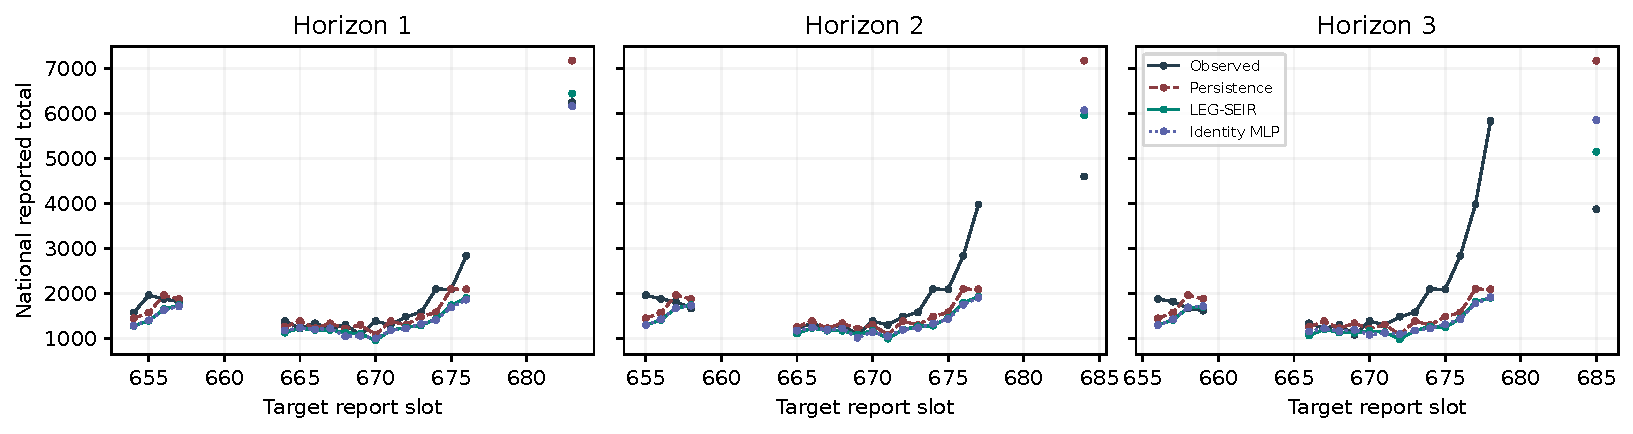
\includegraphics[width=\textwidth]{figures/case_study.pdf}
\caption{All three horizons on the same national-total scale. Neural curves are five-seed ensembles; observed targets and persistence use identical eligible origins. Gaps in source coverage are not bridged. These curves are visualization, not district-pooled seed-mean RMSE. Isolated points remain visible.}\end{figure}
The model does not track every rapid rise: aggregate forecasts can remain below growing observed totals and overshoot after a high recent report. Better pooled error is compatible with those misses. Do not interpret the learned graph as evidence of actual inter-district infection transport.

\begin{figure}[ht]\centering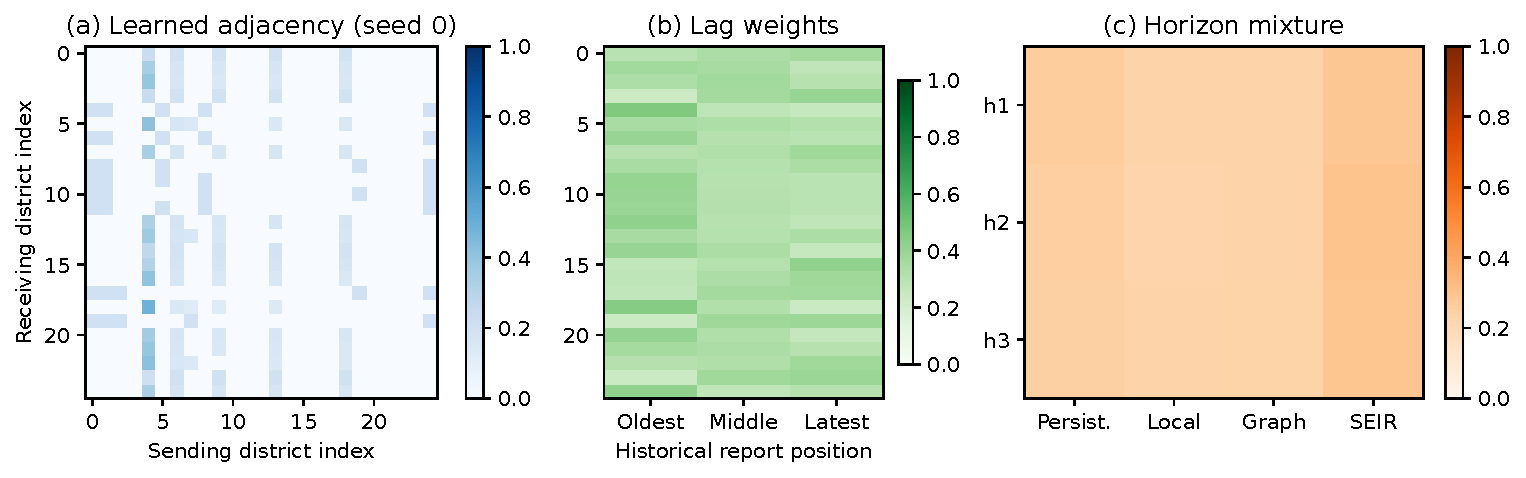
\includegraphics[width=\textwidth]{figures/learned_diagnostics.pdf}
\caption{Seed-zero adjacency, lag and mixture weights. District indices follow the CSV column order. These are descriptive fitted parameters, not measured mobility, disease delays or causal importance. Expert outputs co-adapt. All five seeds' diagnostics are preserved in NPZ exports.}\end{figure}
\begin{figure}[ht]\centering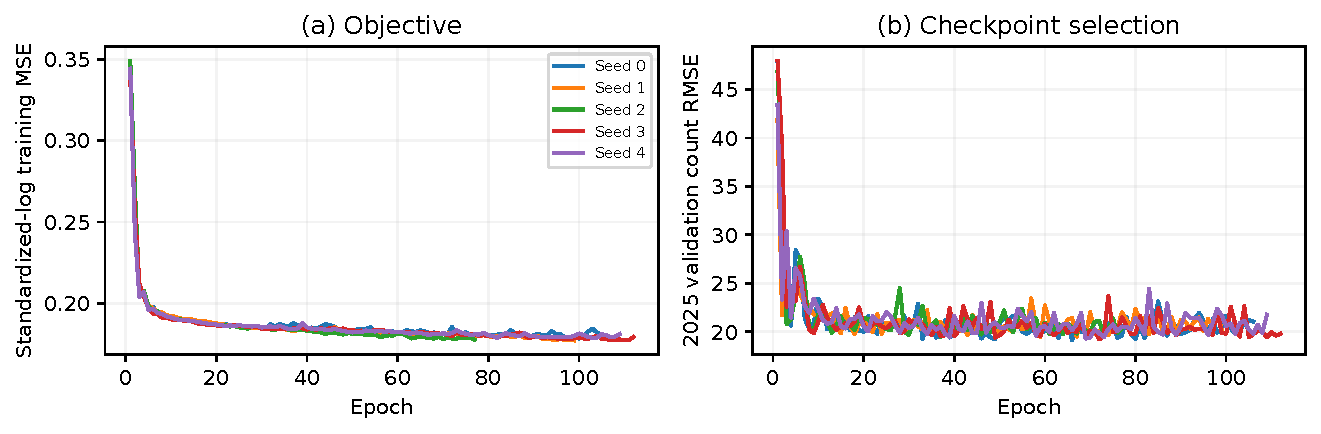
\includegraphics[width=\textwidth]{figures/training_curves.pdf}
\caption{Final LEG-SEIR training loss and 2025 validation RMSE curves. Checkpoints minimize validation count RMSE; epochs after the best point are retained until early stopping. Test scores are not used to select an epoch.}\end{figure}

\clearpage
\section{Reproduction instructions}
\textbf{Public derived-input training.} Run \path{notebooks/LEG_SEIR_train_from_audited_data.ipynb} from the code repository in a new GPU kernel. It downloads pinned audited tables, validates hashes, preserves the original model, loss, fold, learning-rate selection and training cells, and trains all configurations from scratch without reading saved predictions or weights. PDF parsing is skipped; this version has a distinct code/input identity. The recorded study itself was not rerun for this release.

\textbf{Original PDF-to-result workflow.} The frozen notebook in \path{experiments/frozen/Dengue_final_study.ipynb} remains unchanged. Use \path{scripts/retrieve_original_sources.py} with the public original-source manifest to retrieve the exact original files, or extract the team's retained source snapshot beside the notebook. The loader checks every source hash. Files changed or unavailable at their original URLs must be reported, not silently substituted. Source-provider permissions are separate from software licensing.

\textbf{Verify saved evidence.} From a fresh code checkout, install \texttt{requirements-cpu.txt}. Retrieve the pinned snapshot and independently check it using:
\begin{verbatim}
python scripts/fetch_artifacts.py
python scripts/verify.py artifacts/evaluation_outputs.zip artifacts/verified
\end{verbatim}
This checks archive hashes, all neural CPU reloads, targets, scalers, metrics, chronology and LR selection. It does not retrain models or refit ridge. Load only the trusted project checkpoints. Public artifact IDs, immutable HF revision and file SHA256 are recorded in \path{artifacts.lock.json}.

\textbf{Figures and paper.} Run \texttt{python scripts/build\_figures.py} after verification. Exported vector figures and CSV inputs are in \path{figures/publication}. The inspection notebook reads saved results; it is not a training run. Compile \texttt{paper/main.tex} and \texttt{paper/supplement.tex} with the packaged bibliography and figures, or import the Overleaf ZIP. Dataset and code URLs are supplied in the main text rather than bibliography entries.

\section{Reference reproductions: what exists and what is missing}
The historical reproduction collection contains five pinned author-code Weng dengue graph runs and two SEIR mathematics runs, with saved results and scope records. Numerical deviations from published outcomes are disclosed. It does not reproduce every Weng table row or the original traffic/action-recognition tasks behind adapted models. Old notebook task names containing ``exact'' are not evidence of exact numerical equality.

MepoGNN, CausalGNN, IeRNN, M-Graphormer, HeatGNN and Liu--Cao ST-GAT PDFs have been retrieved for this new paper. Their original experiments have not been reproduced here and are not in the main result table. A completed external-method reproduction would require its precise dataset/task and released configuration, or a clearly labelled adaptation. Packaging reference PDFs is not equivalent to that experiment. The reproduction-gap register records this distinction.

\section{Priority, attribution and follow-up tests}
The team proposes the implemented LEG-SEIR configuration. Broad GNN/SEIR coupling, learned spatial dependencies and lagged neighbour memory have precedents. The potential contribution is the compact shared case-lag operator, its dual neural/mechanistic use and historical-to-simulated pressure transition within the specified mixture. An exhaustive equation/code priority audit has not been completed; improved RMSE alone cannot prove methodological novelty.

Required controls for stronger attribution are uniform versus learned lags, latest-only versus history, import gate disabled with neural graph retained, history-only/simulation-only versus transitioning pressure, separate versus shared operators, and matched mixture controls. Test fixed proxy constants and the unresolved-report sensitivity policy. Freeze development-based decisions before genuinely independent future or external evaluation; any further analysis of 2026 stays retrospective. 

\begin{figure}[ht]\centering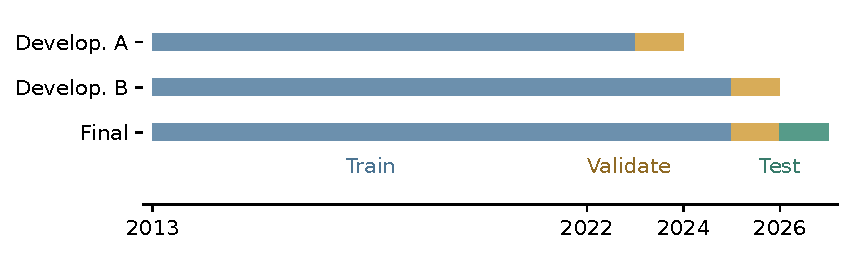
\includegraphics[width=\textwidth]{figures/evaluation_timeline.pdf}
\caption{Chronological development and retrospective final evaluation. Training and checkpoint-selection periods precede scored target years; the previously inspected 2026 case study is not prospective confirmation.}\end{figure}
\section{Extended research context}
\subsection{Encoders and simple forecasting alternatives}
Graph foundations include GCN and GAT~\cite{kipf2017gcn,velickovic2018gat}, while DCRNN uses directed diffusion in traffic forecasting~\cite{li2018dcrnn}. Earlier architecture investigations considered traffic encoders ASTGCN and A3T-GCN~\cite{guo2019astgcn,bai2021a3tgcn}, adaptive action-recognition graph encoders~\cite{shi2019aagcn,shi2020msaagcn}, LSTM~\cite{hochreiter1997lstm} and temporal convolutional networks~\cite{bai2018tcn}. These publications establish their original model designs, not accuracy of adaptations to this dataset. STID and N-BEATS support investigating compact identity-conditioned and MLP-based forecasting designs~\cite{stid2022,nbeats2020}. GLNN studies distillation from graph models to MLPs~\cite{glnn2022}; it does not establish that the reverse direction improves epidemic forecasts. RevIN addresses distribution shift through reversible instance normalization~\cite{revin2022}, and GRU-D incorporates missingness and elapsed time in clinical series~\cite{grud2018}. Neither technique is used in the evaluated LEG-SEIR configuration.

The learned receiver/sender factors have precedents in adaptive spatial forecasting~\cite{wu2019graphwavenet,mtgnn2020,agcrn2020}. The residual graph branch retains a local representation, consistent with the broad residual-learning principle~\cite{resnet2016}; adaptive channel mixing also distinguishes identity and aggregated channels~\cite{acm2022}. Our horizon weights are fixed learned parameters, not the input-conditioned attention of the Transformer~\cite{transformer2017}. These citations describe conceptual context rather than an assertion that our implementation reproduces those architectures.

\subsection{Mechanistic and dengue context}
Physics-informed networks and universal differential equations offer distinct ways of combining neural components with scientific dynamics~\cite{raissi2019pinn,ude2020}. LEG-SEIR uses a differentiable conservative rollout; it does not impose a differential-equation residual penalty. MP-PINN studies a multi-phase epidemic approach~\cite{nguyen2024mppinn}. A recent hybridization study reports limitations under partial observation and nonstationarity~\cite{hybrid2026}; this preprint is preliminary context, not confirmation of failure modes in our experiment.

Graph epidemic work includes EpiGNN, STAN, MPSTAN, IeRNN, CausalGNN, MepoGNN, HeatGNN and M-Graphormer~\cite{epignn2022,stan2020,mpstan2023,iernn2020,causalgnn2022,mepognn2023,heatgnn2024,mgraphormer2025}. EISTGNN and MechGNN-Epi are additional published hybrid-model references~\cite{eistgnn2025,mechgnn2026}; their bibliographic records were checked, but their original experiments were not reproduced here. Without matched reruns, none supplies a numerical superiority claim for LEG-SEIR. Close dengue references include Weng et al., DengueGNN and the Sri Lankan covariate compartmental model~\cite{weng2024graph,gulmohamed2026denguegnn,liu2025seirlstm}, alongside lagged neighbourhood forecasting~\cite{liucao2026}. Vector--host modelling and sensitivity analyses provide context for mechanisms omitted by our human-only proxy decoder~\cite{seirsei2022,phaijoo2018sensitivity}; the basic SEIR equations are also documented in official university notes~\cite{gopalakrishnan2020seir}.

\subsection{Evaluation and attribution}
Sri Lankan epidemic context is documented by Tissera et al.~\cite{tissera2020severe}. Dengue forecasting challenges and comparative evaluations motivate transparent outcome definitions~\cite{johansson2019challenge,johansson2016evaluation}. Persistence initialization~\cite{haugsdal2023persistence}, simple forecasting baselines~\cite{zeng2023nlinear}, forecast-accuracy measures~\cite{hyndman2006accuracy}, dependent-data resampling~\cite{kunsch1989bootstrap} and selection bias~\cite{cawley2010selection} motivate the controls and limits described in the manuscript. Adam is the optimizer used in the recorded runs~\cite{kingma2015adam}. Citations do not establish that this particular combination is the first of its kind; novelty remains confined to the proposed computation and the reported comparisons.

\bibliographystyle{IEEEtran}
\bibliography{references}
\end{document}
